\documentclass[11pt,a4paper]{article}
\usepackage[T1]{fontenc}
\usepackage[utf8]{inputenc}
\usepackage[french]{babel}
\usepackage{lmodern}
\usepackage[margin=2.2cm]{geometry}
\usepackage{amsmath,amssymb}
\usepackage{booktabs}
\usepackage{graphicx}
\usepackage{float}
\usepackage[hidelinks]{hyperref}
\usepackage{xcolor}

\setlength{\emergencystretch}{3em}
\newcommand{\code}[1]{\texttt{#1}}
\graphicspath{{figs/}}

\title{Moteur d'échecs matriciel sur GPU\\[2pt]
\large Débit brut, recherche, alpha-bêta par lots et matchs contre Stockfish\\
\normalsize Rapport d'incrément et plan du suivant}
\author{Projet \code{chess-gpu}, branche \code{claude/zen-pasteur-vjg9yx}}
\date{24 novembre 2026}

\begin{document}
\maketitle

\begin{abstract}
On porte sur GPU (NVIDIA RTX PRO 6000 Blackwell, 96~Go) le moteur d'échecs matriciel du dépôt,
où chaque coup est une matrice $T$ telle que $b' = T\,b$. La génération des coups légaux tourne
entièrement par lots de tenseurs. Le perft atteint $5{,}1\cdot 10^{10}$ nœuds/s, soit 157 fois
\code{go perft} de Stockfish~16 sur un thread. En jeu, une recherche negamax pleine largeur
calcule 100 à 300 fois plus de positions que Stockfish, mais ne voit que 4 à 6 demi-coups : elle
plafonne vers 1500--1700 Elo de Stockfish bridé. On formule alors un équivalent matriciel de
l'alpha-bêta, par fenêtres $[\alpha,\beta]$ et vagues de fils traitées par lots, dont on démontre
la convergence et que l'on mesure. À temps égal, il gagne 1 à 3 demi-coups et garde exactement la
valeur minimax. Trois agents ont été consultés. On confronte ici leurs hypothèses aux mesures GPU
et l'on fixe le plan du prochain incrément.
\end{abstract}

\tableofcontents

\section{Objectif}
La question de départ est double. \emph{Combien de positions peut-on simuler par seconde sur un
GPU avec le calcul matriciel du dépôt, et peut-on aller plus vite que Stockfish ?} Puis, après
les premiers matchs : \emph{comment obtenir l'équivalent d'un alpha-bêta par du pur calcul
matriciel, avec un critère de convergence ?} Ces deux questions ont des réponses différentes. La
première porte sur le débit, la seconde sur la quantité de calcul utile. Tout le rapport tient
dans l'écart entre les deux.

\section{Glossaire}
\begin{description}
\item[Perft] Nombre exact de feuilles de l'arbre des coups légaux à une profondeur donnée. Les
valeurs de référence publiées valident un générateur de coups, et la vitesse de calcul mesure le
débit brut.
\item[Kiwipete] Position de test de Peter McKenzie
(\code{r3k2r/p1ppqpb1/bn2pnp1/3PN3/1p2P3/2N2Q1p/PPPBBPPP/R3K2R w KQkq -}). Elle réunit les quatre
roques, des prises en passant, des clouages et des échecs, avec 48 coups légaux au premier
demi-coup. Son perft à la profondeur 6 vaut 8\,031\,647\,685.
\item[Pleine largeur] Minimax qui développe tous les coups à chaque niveau, sans élagage.
\item[Alpha-bêta] Minimax qui abandonne un sous-arbre dès qu'il ne peut plus influencer le choix,
grâce à une fenêtre $[\alpha,\beta]$. Avec un tri parfait, il ne visite qu'environ $b^{d/2}$
nœuds au lieu de $b^d$.
\item[Fail-soft] Variante d'alpha-bêta qui renvoie la meilleure borne trouvée, même hors de la
fenêtre. La valeur est exacte si $\alpha<v<\beta$, et sinon c'est une borne du bon côté.
\item[YBW] \emph{Young Brothers Wait} (Feldmann) : parallélisation de l'alpha-bêta où l'on
cherche d'abord le premier fils seul, l'aîné, puis tous les autres, les cadets, en parallèle avec
la borne qu'il a fournie.
\item[Vagues] Ici, découpe des fils d'un nœud, triés, en groupes de rangs traités par lots
successifs : YBW, 1-2-4 ou hybride.
\item[Quiescence] Prolongement de la recherche aux seules prises, jusqu'à une position calme, pour
éviter l'effet d'horizon. Le \emph{stand pat} permet au camp au trait de ne pas prendre.
\item[MVV/LVA] \emph{Most Valuable Victim, Least Valuable Attacker} : on joue d'abord les prises
de la pièce la plus chère par la pièce la moins chère.
\item[Facteur de branchement effectif] Rapport $N_d/N_{d-1}$ des nœuds visités entre deux
profondeurs. Il vaut environ 35 en pleine largeur et tend vers $\sqrt{35}\approx6$ pour un
alpha-bêta parfaitement trié.
\end{description}

\section{Génération des coups sur GPU}
\paragraph{Données.} Un lot de $N$ positions, toutes avec le même camp au trait, est porté par
trois tenseurs : les plateaux $B\in\mathbb{Z}^{N\times 65}$ en \code{int8} (64 cases et une
sentinelle toujours nulle), les droits de roque $(N,4)$ et la case en passant $(N,)$. Les coups
pseudo-légaux sont 70 plans booléens $(N,70,8,8)$ : 8 directions $\times$ 7 distances pour les
pièces glissantes et le roi, 8 sauts de cavalier, 4 plans de pion, 2 roques. Chaque plan s'obtient
par décalages et opérations élémentaires, comme dans \code{engine.py}. Un \code{nonzero} décode
les plans en coups au format \code{reduced.pack}, et \code{apply\_moves} calcule $b'=Tb$ par un
\code{gather} et un \code{scatter}.

\paragraph{Légalité.} Le test d'échec ne calcule plus les attaques de tout le camp adverse. Il
lit 74 cases depuis le roi : 8 rayons de 7 cases, 8 sauts de cavalier, 8 voisins et 2 cases de
pion, en un seul \code{gather}. Sur CPU, perft passe de $2{,}4\cdot10^5$ à $8\cdot10^5$
nœuds/s.

\paragraph{Fusion.} \code{torch.compile} fusionne les centaines d'opérations élémentaires. Sur
GPU, il divise par 7 la génération et par 23 le test d'échec. Un sous-agent a ensuite écrit un
noyau CUDA (\code{gpu\_kernels.py}, compilé par CuPy) : un fil par position, des bitboards, les
clouages et les échecs calculés une fois, puis une écriture compactée des enfants. Un test impose
l'égalité exacte, ordre compris, avec le chemin \code{torch} sur les positions de 300 parties
aléatoires.

\begin{figure}[H]
\centering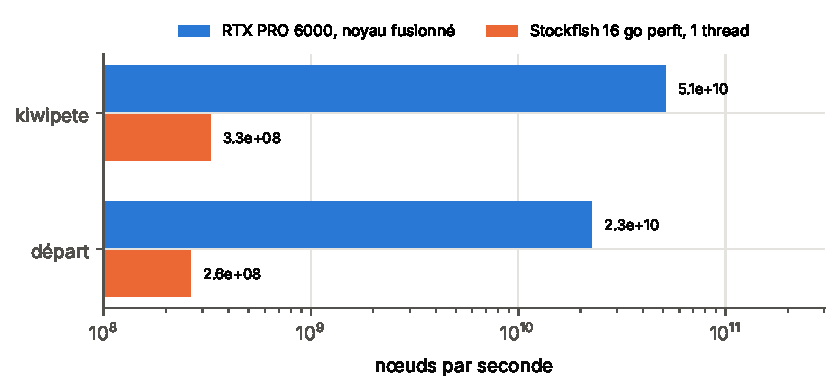
\includegraphics[width=0.85\linewidth]{perft.pdf}
\caption{Perft profondeur 6 : noyau fusionné sur RTX PRO 6000 contre \code{go perft} de
Stockfish~16, un thread. Kiwipete donne 8\,031\,647\,685 nœuds, la valeur de référence, en
0{,}16~s.}
\end{figure}

\paragraph{Vérification.} Les perft des cinq positions de référence de chessprogramming.org sont
exacts, et les ensembles de coups légaux sont identiques à ceux de python-chess
(\code{test\_gpu\_engine}).

\section{Recherche pleine largeur et matchs}
La recherche est un negamax pleine largeur, suivi d'une quiescence sur les prises (seulement
celles où la victime vaut au moins l'attaquant, MVV/LVA). L'évaluation additionne le matériel et
des tables de cases. Trois versions se sont succédé.
\begin{itemize}
\item \textbf{v1} (\code{torch} + compile) : l'arbre est stocké niveau par niveau, environ
$4\cdot10^7$ nœuds/s.
\item \textbf{v2} (noyau CUDA) : environ $2{,}7\cdot10^8$ nœuds/s. La profondeur reste bornée par
la mémoire, la profondeur 6 demandant environ 160~Go.
\item \textbf{v3} (récursive par lots) : comme perft, chaque niveau ne garde qu'un lot. La mémoire
tombe de 93 à 11{,}6~Go, et une itération peut être interrompue à la pendule.
\end{itemize}

Les matchs se jouent en 3+0 contre Stockfish~16 local (1 thread, Hash 256~Mo), bridé par
\code{UCI\_LimitStrength}, deux parties par niveau, couleurs alternées. python-chess arbitre.

\begin{table}[H]
\centering\small\begin{tabular}{lcccccccrrrr}
\toprule
série & 1320 & 1500 & 1700 & 1900 & 2200 & 2500 & max & total & nœuds/s & prof. & prof. SF\\
\midrule
v1-torch & 1/2 & 1/2 & 1/2 & 0/2 & 0{,}5/2 & 0/2 & 0/2 & 3{,}5/14 & $4{,}0\cdot 10^{7}$ & 4{,}2 & 35\\
v2-noyau-temps & 2/2 & 1/2 & 0{,}5/2 & 0/2 & 1/2 & 0/2 & 0/2 & 4{,}5/14 & $2{,}7\cdot 10^{8}$ & 4{,}9 & 34\\
v3-recursif & 1{,}5/2 & 2/2 & 0/2 & 0/2 & -- & -- & -- & 3{,}5/8 & $2{,}7\cdot 10^{8}$ & 5{,}3 & 36\\
\bottomrule
\end{tabular}

\caption{Points marqués par niveau d'Elo de Stockfish. Les trois dernières colonnes donnent les
médianes par partie de notre débit, de notre profondeur et de celle de Stockfish.}
\end{table}

\begin{figure}[H]
\centering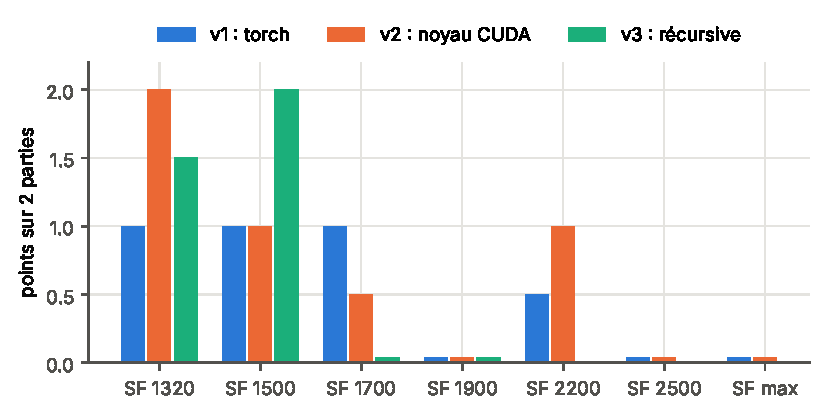
\includegraphics[width=0.85\linewidth]{scores.pdf}
\caption{Score par niveau (2 parties par niveau).}
\end{figure}

\begin{figure}[H]
\centering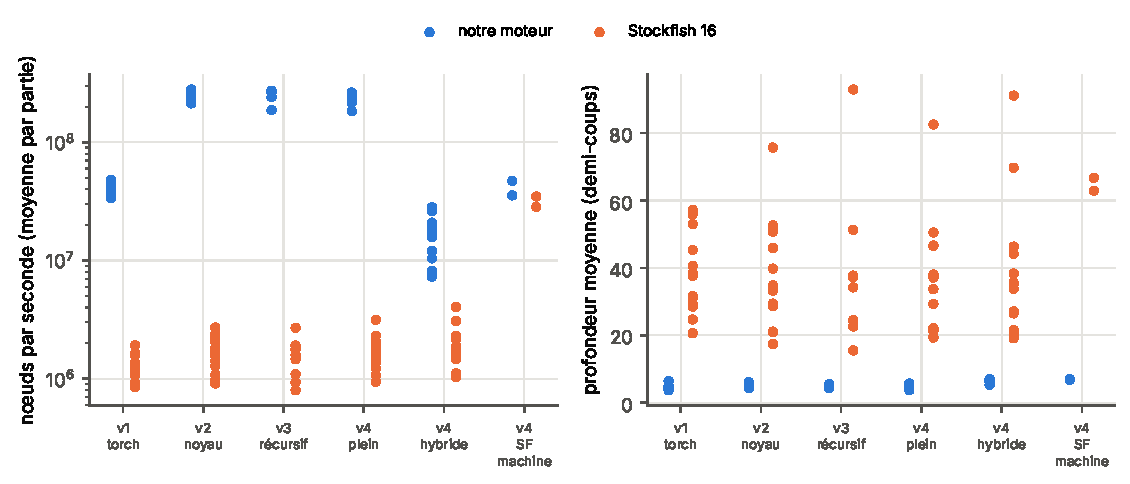
\includegraphics[width=0.95\linewidth]{vitesse_profondeur.pdf}
\caption{Par partie, débit moyen (échelle log) et profondeur moyenne des deux moteurs.}
\end{figure}

\paragraph{Lecture.} On calcule 100 à 300 fois plus de positions que Stockfish, mais il voit
17 à 93 demi-coups contre 4 à 6. L'élagage domine la force brute : la pleine largeur paie un
facteur proche de $b\approx35$ par demi-coup. Deux parties par niveau donnent une tendance, pas un
Elo. De plus, les niveaux \code{UCI\_Elo} ne sont calibrés qu'en 60~s~+~0{,}6~s (wiki UCI de
Stockfish), alors que ces matchs sont en 3+0 ; d'où le préréglage \code{uci-elo} de la
section~\ref{sec:v4}.

\section{Un alpha-bêta matriciel}
\subsection{Formulation}
On remplace la valeur d'un nœud par un intervalle $[L,U]$, ou par une fenêtre
$[\alpha,\beta]$ en version fail-soft. En negamax, la remontée d'un niveau s'écrit
\[
L(p)=\max_{c\in\mathrm{fils}(p)} -U(c),\qquad U(p)=\max_{c\in\mathrm{fils}(p)} -L(c),
\]
c'est-à-dire un produit matrice-vecteur dans le semi-anneau $(\max,+)$ :
$[L;U]\leftarrow A\otimes[-U;-L]$, où $A$ est l'adjacence parent--fils, creuse, valant $0$ sur
les arêtes et $-\infty$ ailleurs. Sur GPU, c'est exactement le \code{scatter\_reduce(amax)} déjà
employé. La descente passe les fenêtres aux fils, $\alpha(c)=-\beta(p)$ et
$\beta(c)=-\max(\alpha(p),\mathrm{best}(p))$, par un \code{gather}. Un parent est \emph{coupé}
dès que $\mathrm{best}(p)\ge\beta(p)$.

\subsection{Convergence}
\begin{itemize}
\item \textbf{Validité} : $L\le v\le U$ en tout nœud, par récurrence sur la hauteur.
\item \textbf{Monotonie} : développer un nœud ne fait que resserrer, $L$ ne décroît jamais et $U$
ne croît jamais.
\item \textbf{Terminaison} : sur un arbre fini, chaque itération non terminale développe au moins
un nœud. Au point fixe, la racine vérifie $L=U=v_{\text{minimax}}$. La convergence est monotone et
finie, au sens d'une itération de Kleene sur un treillis fini. Ce n'est pas une contraction : sans
facteur d'escompte, l'écart $U-L$ procède par sauts, et l'agent algébrique a mesuré à la racine
de Kiwipete la suite $[-\infty,\infty]$, $[-165,\infty]$, $[-165,735]$, $[400,400]$.
\item \textbf{Critère de décision à la racine} : le meilleur coup est prouvé dès que
$L(\text{meilleur})\ge U(\text{autres})$. En pratique, ce critère n'est atteint qu'en fin
d'itération : c'est prouver que les autres coups sont moins bons qui coûte.
\item \textbf{Lien avec \code{retro.py}} : c'est le même opérateur que l'analyse rétrograde, mais
appliqué au graphe d'états complet sur le treillis \{perte, nulle, gain\}, où il converge en au
plus DTM$_{\max}$ itérations.
\end{itemize}

\subsection{Par lots : les vagues}
Les bornes n'existent qu'une fois un premier fils résolu. Les fils de chaque parent, triés par
évaluation statique, sont donc cherchés par \emph{vagues de rangs}. Seuls les parents non coupés
lancent la vague suivante. On a implémenté trois découpes dans \code{Searcher(prune=True,
waves=\ldots)} :
\begin{itemize}
\item \textbf{YBW} : l'aîné seul, puis tous les cadets ;
\item \textbf{1-2-4} : les rangs $\{0\}, \{1,2\}, \{3..6\}, \{7..14\}, \ldots$ ;
\item \textbf{hybride} : l'aîné, puis les rangs 1 à 3, puis le reste.
\end{itemize}
En quiescence, le \emph{stand pat} coupe avant toute prise. À la racine, le coup de l'itération
précédente passe en premier, avec la fenêtre pleine. Un test impose que le score soit identique à
celui de la pleine largeur pour toutes les découpes, sur CPU et sur GPU, et chaque mesure
ci-dessous le vérifie par assertion.

\subsection{Mesures sur RTX PRO 6000}
\begin{table}[H]
\centering\scriptsize\begin{tabular}{lccccc}
\toprule
position & d & pleine largeur & YBW & hybride & 1-2-4\\
\midrule
départ & 4 & $2{,}71\cdot 10^{5}$ en 0{,}01~s & $1{,}33\cdot 10^{4}$ en 0{,}03~s & $1{,}33\cdot 10^{4}$ en 0{,}04~s & $1{,}32\cdot 10^{4}$ en 0{,}05~s\\
 & 6 & -- & $3{,}41\cdot 10^{6}$ en 0{,}15~s & $8{,}71\cdot 10^{5}$ en 0{,}39~s & $7{,}46\cdot 10^{5}$ en 1{,}18~s\\
kiwipete & 4 & $1{,}34\cdot 10^{9}$ en 4{,}17~s & $6{,}95\cdot 10^{5}$ en 0{,}04~s & $1{,}99\cdot 10^{5}$ en 0{,}07~s & $1{,}83\cdot 10^{5}$ en 0{,}12~s\\
 & 6 & -- & $1{,}54\cdot 10^{8}$ en 0{,}90~s & $5{,}70\cdot 10^{6}$ en 0{,}56~s & $4{,}94\cdot 10^{6}$ en 1{,}82~s\\
italienne & 4 & $6{,}14\cdot 10^{6}$ en 0{,}03~s & $3{,}42\cdot 10^{5}$ en 0{,}04~s & $1{,}09\cdot 10^{5}$ en 0{,}09~s & $9{,}92\cdot 10^{4}$ en 0{,}24~s\\
 & 6 & -- & $1{,}35\cdot 10^{8}$ en 0{,}83~s & $4{,}32\cdot 10^{6}$ en 0{,}81~s & $3{,}30\cdot 10^{6}$ en 3{,}72~s\\
gambit-dame & 4 & $1{,}58\cdot 10^{7}$ en 0{,}06~s & $4{,}56\cdot 10^{6}$ en 0{,}06~s & $3{,}78\cdot 10^{5}$ en 0{,}08~s & $3{,}48\cdot 10^{5}$ en 0{,}21~s\\
 & 6 & -- & $3{,}47\cdot 10^{9}$ en 15{,}94~s & $7{,}78\cdot 10^{7}$ en 1{,}20~s & $1{,}77\cdot 10^{7}$ en 4{,}26~s\\
finale-tours & 4 & $2{,}92\cdot 10^{5}$ en 0{,}01~s & $1{,}47\cdot 10^{5}$ en 0{,}03~s & $2{,}03\cdot 10^{4}$ en 0{,}05~s & $1{,}58\cdot 10^{4}$ en 0{,}10~s\\
 & 6 & -- & $2{,}80\cdot 10^{7}$ en 0{,}30~s & $1{,}28\cdot 10^{6}$ en 0{,}46~s & $7{,}48\cdot 10^{5}$ en 1{,}79~s\\
\bottomrule
\end{tabular}

\caption{Nœuds générés et temps mur à profondeur fixe, quiescence 4. Le score est identique dans
chaque ligne.}
\end{table}

\begin{figure}[H]
\centering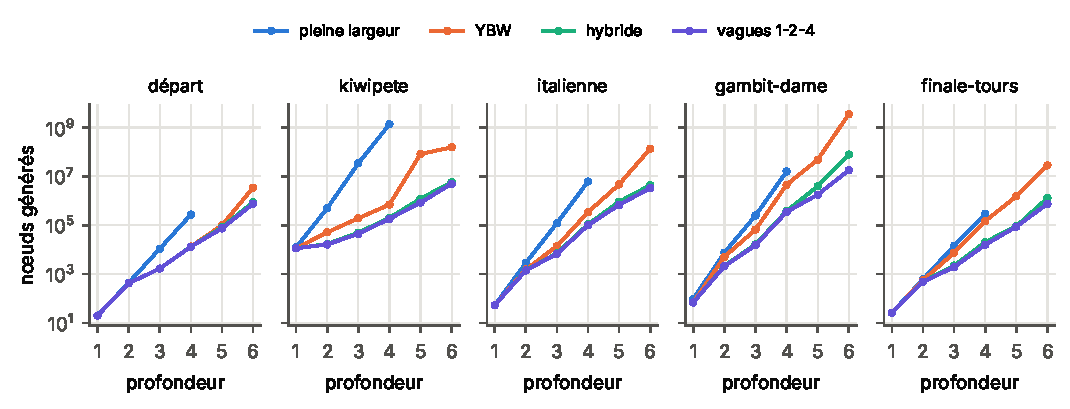
\includegraphics[width=\linewidth]{alphabeta_noeuds.pdf}
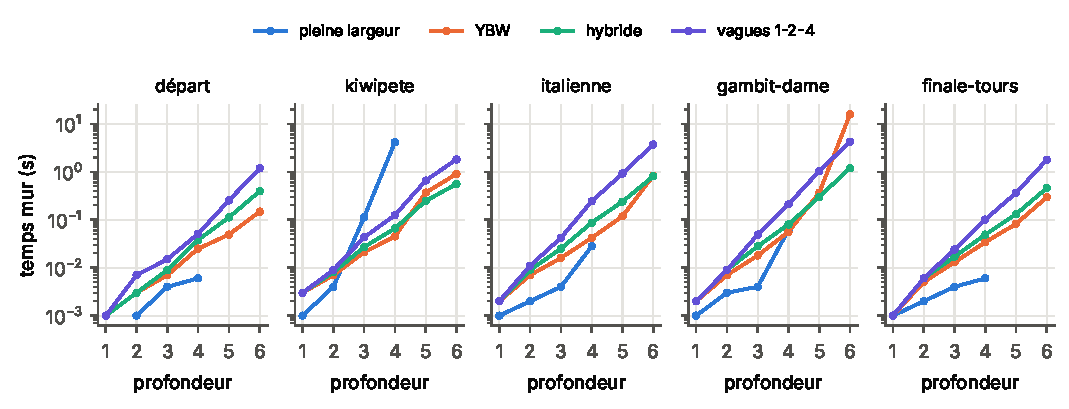
\includegraphics[width=\linewidth]{alphabeta_temps.pdf}
\caption{Nœuds et temps mur par profondeur, échelle log, quiescence 4.}
\end{figure}

\begin{table}[H]
\centering\small\begin{tabular}{lcccc}
\toprule
position & pleine largeur & YBW & hybride & 1-2-4\\
\midrule
départ & 6 (0{,}9~s) & 8 (8{,}7~s) & 8 (4{,}5~s) & 7 (3{,}7~s)\\
kiwipete & 4 (4{,}2~s) & 6 (9{,}0~s) & 7 (5{,}6~s) & 6 (9{,}0~s)\\
italienne & 5 (1{,}0~s) & 6 (9{,}0~s) & 7 (3{,}3~s) & 6 (3{,}7~s)\\
gambit-dame & 5 (2{,}0~s) & 5 (9{,}0~s) & 6 (9{,}0~s) & 6 (4{,}2~s)\\
finale-tours & 6 (9{,}0~s) & 7 (2{,}1~s) & 9 (8{,}5~s) & 6 (1{,}8~s)\\
\bottomrule
\end{tabular}

\caption{Profondeur complète atteinte avec un budget de 3~s par coup (plafond dur de 9~s), et
temps mur réellement consommé.}
\end{table}

\paragraph{Ce que montrent les mesures.}
\begin{enumerate}
\item L'élagage est massif avec quiescence. Sur Kiwipete en profondeur 4, YBW garde 0{,}05~\% des
nœuds de la pleine largeur et passe de 4{,}17~s à 0{,}045~s.
\item Moins de nœuds ne veut pas dire plus rapide sur GPU. La découpe 1-2-4 coupe 10 à 200 fois
plus de nœuds que YBW, mais ses lots sont trop petits : le débit tombe de $\sim2\cdot10^8$ à
$\sim3\cdot10^6$ nœuds/s, et elle est la plus lente sur quatre positions sur cinq.
\item YBW explose quand le tri se trompe. Sur le Gambit-Dame en profondeur 6, il génère
$3{,}5\cdot10^9$ nœuds en 15{,}9~s, contre 1{,}2~s pour l'hybride.
\item L'hybride est le meilleur compromis. Il n'a jamais de pathologie et atteint, en 3 à 6~s, la
profondeur 8 depuis le départ et 7 sur Kiwipete et l'Italienne, là où la pleine largeur
s'arrêtait à 4--6.
\item Les itérations interrompues coûtent cher. La prédiction du coût de l'itération suivante se
trompe, et l'on consomme le plafond dur (9~s pour 3~s de budget).
\end{enumerate}

\section{Avis des agents et confrontation aux mesures}
Trois agents indépendants ont été consultés : l'un sur la formulation algébrique, un autre sur les
algorithmes par lots, le dernier en avocat du diable. Les deux premiers ont reçu les mesures GPU
et révisé leur avis.

\begin{table}[H]
\centering\small
\begin{tabular}{p{5.2cm}p{4.2cm}p{5.2cm}}
\toprule
Hypothèse & Agent & Verdict des mesures GPU\\
\midrule
L'intervalle $[L,U]$ remonte par $(\max,+)$, avec une convergence monotone finie mais sans
contraction & algébrique & Confirmé. Même score que le minimax partout, et l'écart évolue par
sauts.\\
YBW élague massivement, mais reste sensible au tri & algébrique & Confirmé : 0{,}05~\% des nœuds
sur Kiwipete, et explosion à $3{,}5\cdot10^9$ nœuds sur le Gambit-Dame.\\
Les vagues 1-2-4 donnent un facteur de branchement effectif de 8,6 à 9,7 et environ 8 demi-coups
en 3~s & lots & Nœuds confirmés. Temps infirmé : le débit est divisé par 30 à 100, car les lots
sont trop petits.\\
L'élagage exact rapporte $+1{,}5$ à $+2{,}5$ demi-coups & lots & Confirmé : $+2$ à $+3$ avec
l'hybride.\\
Un bassin global de nœuds prêts réglerait le débit & lots & Rétrogradé par l'agent lui-même : le
chemin critique compte des milliers de pas à $d=8$.\\
\bottomrule
\end{tabular}
\caption{Hypothèses des agents et verdict.}
\end{table}

\noindent\textbf{Ce sur quoi les agents convergent après les mesures.}
\begin{enumerate}
\item \emph{Le tri des coups d'abord}. L'explosion de YBW vient d'un nœud de coupe dont l'aîné ne
coupe pas : ses $b-1$ frères partent alors avec la même fenêtre. Il faut placer les prises en
MVV/LVA en tête, puis tenir des tables « killer » et d'historique sous forme de tenseurs, mises à
jour par \code{scatter\_add} sur les coups qui coupent.
\item \emph{Des vagues adaptatives}. On échelonne finement tant que le sous-arbre évité est grand,
c'est-à-dire tant que le nombre de fils restants $\times 9^{\,rem-1}$ dépasse un seuil $S$ entre
$10^5$ et $10^6$, à calibrer. Sinon, on lance tous les rangs d'un coup.
\item \emph{La gestion du temps}. On prédit le coût par le facteur de branchement effectif mesuré
$N_d/N_{d-1}$, et l'on garde le résultat partiel. Un coup racine qui a battu le précédent sous la
fenêtre $(-\infty,-\text{score})$ est déjà valide.
\item \emph{La table de transposition en dernier}. Son gain potentiel est le plus grand, mais les
collisions de \code{scatter} et la mémoire restent à concevoir.
\item \emph{L'élagage non exact} (LMR, coup nul) ensuite. L'égalité avec le minimax ne tient
plus, et il faut valider par des parties.
\end{enumerate}

\noindent\textbf{Grandeurs de convergence à journaliser} : le facteur de branchement effectif
$N_d/N_{d-1}$, à situer entre $\sqrt b$ et $b$ ; le taux de coupe en première vague, qui mesure
directement la qualité du tri ; enfin, la stabilité entre profondeurs, c'est-à-dire la constance
du coup racine et la valeur de $|v_d-v_{d-1}|$.

\subsection*{Avocat du diable}
Rapport en attente.


\section{Matchs dans les conditions de référence}\label{sec:v4}
Les séries v4 se jouent dans les conditions de calibration de \code{UCI\_Elo} : 60~s~+~0{,}6~s,
Stockfish~16 sur 1 thread avec Hash 16~Mo (préréglage \code{uci-elo}). Toutes ont tourné sur la
même RTX PRO 6000. Le tableau donne les médianes par partie : débit, profondeur moyenne de notre
moteur et profondeur de Stockfish.

\begin{table}[H]
\centering\scriptsize\begin{tabular}{lcccccccrrrr}
\toprule
série & 1320 & 1500 & 1700 & 1900 & 2200 & 2500 & max & total & nœuds/s & prof. & prof. SF\\
\midrule
\\
\bottomrule
\end{tabular}

\caption{Séries v4. \code{v4-hybride-ucielo} a été jouée avant le correctif de racine décrit
ci-dessous ; \code{v4b} est la même série après correctif. \code{v4-hybride-machine} oppose
l'hybride à Stockfish sur toute la machine (30 threads, Hash 8~Go).}
\end{table}

\begin{figure}[H]
\centering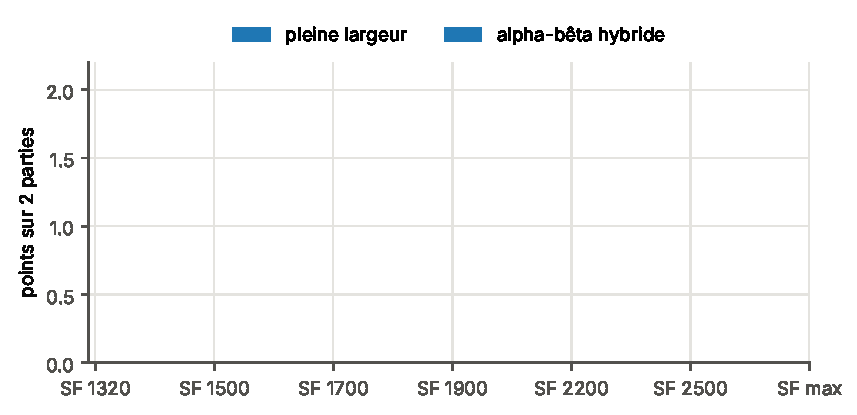
\includegraphics[width=0.85\linewidth]{scores_ucielo.pdf}
\caption{Conditions de calibration (60~s~+~0{,}6~s) : alpha-bêta hybride corrigé contre pleine
largeur, deux parties par niveau.}
\end{figure}

\paragraph{Un bug trouvé par les matchs.} La première série hybride a perdu ses quatre parties,
dont des mats en 22 et 25 demi-coups, alors qu'elle cherchait plus profond (6{,}4 en moyenne
contre 4{,}8). La cause était à la racine. Les coups autres que le premier sont cherchés avec la
fenêtre $(-\infty,-s_0)$, et leur score fail-soft n'est alors qu'une borne haute, souvent égale à
$s_0$. Sur une égalité, \code{argmax} renvoyait le premier indice du tableau, parfois un coup
réfuté. Le test d'équivalence ne comparait que le score, pas le coup joué : il ne pouvait pas le
voir. Le correctif place ces bornes strictement sous $s_0$. Un nouveau test exige que la valeur
exacte du coup joué égale la valeur minimax ; il échouait avant le correctif.

\paragraph{Résultats après correctif.}
\begin{itemize}
\item L'alpha-bêta hybride marque \textbf{7{,}5/14}, contre 5{,}5/14 pour la pleine largeur. C'est
le meilleur total de toutes les séries, avec 1{,}5/2 contre Stockfish 2200 et 0{,}5/2 contre 2500.
Il cherche à 6{,}4 demi-coups en médiane, contre 4{,}8, avec un débit 13 fois plus faible
($1{,}9\cdot10^7$ contre $2{,}5\cdot10^8$ nœuds/s).
\item Sur 14 parties par série, l'écart de 2 points ne départage rien statistiquement : l'erreur
type de l'écart entre deux séries vaut environ $\pm130$ Elo. Il va dans le sens prévu par l'avocat du diable, pour qui la
profondeur est le facteur limitant.
\item Face à Stockfish sur toute la machine, Stockfish calcule $2{,}8$ à $3{,}5\cdot10^7$ nœuds/s,
contre $3{,}6$ à $4{,}7\cdot10^7$ pour nous. L'avantage de débit brut tombe à environ 1{,}3, alors
qu'il était de 100 à 300 face à un seul thread. Stockfish voit 63 à 67 demi-coups, nous 7. Les deux
parties sont perdues.
\end{itemize}


\section{Ressources de Stockfish}
Les deux seules références officielles vérifiées sont les suivantes.
\begin{itemize}
\item La commande \code{bench} de Stockfish utilise les réglages par défaut du moteur : 1 thread
et Hash 16~Mo. On l'a lu dans le moteur ; elle donne ici environ $1{,}05\cdot10^6$ nœuds/s sur le
CPU du conteneur.
\item La calibration de \code{UCI\_Elo} se fait en 60~s~+~0{,}6~s, ancrée sur CCRL 40/4 (wiki UCI
de Stockfish).
\end{itemize}
Le préréglage \code{--preset uci-elo} de \code{match.py} reproduit les deux. Le préréglage
\code{--preset machine} donne à Stockfish tous les cœurs sauf deux, épinglés par \code{taskset},
avec Hash 8~Go. Notre moteur garde les deux cœurs restants. Les API Stockfish en ligne ont été
écartées : elles plafonnent à une profondeur de 15 ou 18 (chiffres de 2024) et ajoutent la
latence réseau à la pendule.

\section{Plan du prochain incrément}
\begin{enumerate}
\item \textbf{Tri des coups.} Prises MVV/LVA en tête, puis killer et historique en tenseurs.
\emph{Validation} : le taux de coupe en première vague, et les nœuds du Gambit-Dame en
profondeur 6 sous YBW.
\item \textbf{Vagues adaptatives} au seuil $S$. \emph{Validation} : le temps mur à profondeur
fixe sur les cinq positions, qui doit être meilleur que l'hybride partout.
\item \textbf{Gestion du temps} : prédiction par $N_d/N_{d-1}$ et résultat partiel conservé.
\emph{Validation} : temps consommé sur temps budgété, qui doit rester sous 1{,}5.
\item \textbf{Matchs statistiques} en préréglage \code{uci-elo}, avec au moins 100 parties par
niveau et un intervalle de confiance sur l'Elo. Deux parties ne départagent rien.
\item \textbf{Table de transposition} sur GPU, puis LMR et coup nul validés par des parties.
\item \textbf{Volet rétrograde} : porter \code{retro.predecessors} sur GPU (la préimage
$b=R\,b'+c\,e_t$ est un \code{gather}/\code{scatter}), et brancher les buts de \code{impose.py},
comme le mat étouffé, en fonction d'évaluation minimisée en minimax. Cela répond à la question
de la convergence vers une position finale imposée.
\end{enumerate}

\section{Reproductibilité et coûts}
\begin{itemize}
\item Tests : \code{python -m unittest src.matrix\_chess.test\_gpu\_engine -v}, sur CPU et sur
GPU.
\item Perft : \code{python -m src.matrix\_chess.bench\_gpu 6}.
\item Matchs : \code{python -m src.matrix\_chess.match --prune --waves hybride --preset uci-elo}.
\item Données : \code{results/matrix\_chess/} (\code{summary.csv}, \code{games.txt},
\code{ab\_gpu.csv}, \code{perft\_gpu.csv}).
\item Figures et tableaux : \code{python docs/rapport\_gpu/gen\_figures.py}.
\end{itemize}
Les pods Runpod RTX PRO 6000 coûtent 2{,}69~\$/h en cloud sécurisé. Un hôte communautaire à
1{,}69~\$/h a été écarté : son pilote renvoyait \code{cuInit} = 999. Les coups de la série v3 sont
perdus, parce que le disque du conteneur est effacé à l'arrêt d'un pod sans volume.

\end{document}
